% !!!!!!!!!!!!!!!!!!   ВНИМАНИЕ !!!!!!!!!!!!!!!!!!!!!!!!!!!!!!!!!!!!!!!!!!!!!!!!!!!!!!!!!
% Заголовки разделов формируются при помощи команд \section{}, \subsection{}, \subsubsection{}
% Не используйте уровень вложенности заголовков больше трех!
% -----------------------------
% Для оформления теорем, лемм, следствий используйте окружения 
% Def     - Определение
% Teor    - Теорема
% Lem     - Лемма
% Predl   - Предложение
% Ass     - Утверждение
% Cor     - Следствие
% Example - Пример
% -----------------------------
% Доказательство теоремы начинается командой \proof и завершается командой \endproof
% -----------------------------
% Литература помещается в окружение biblio.

\documentclass[11pt, oneside, a4paper]{article}
%\usepackage[cp1251]{inputenc} % кодировка
\usepackage[utf8]{inputenc} % кодировка
\usepackage[english, russian]{babel} % Русские и английские переносы
\usepackage{graphicx}          % для включения графических изображений
\usepackage[unicode, pdftex]{hyperref}
\usepackage{cite}              % для корректного оформления литературы
\usepackage{enumitem}
\usepackage{amsmath,amsthm,amssymb}
\usepackage{mathtext}


%стилевой пакет
\usepackage{schoolseminar2022}                                


%\renewcommand{\thefootnote}{*}\footnote{Работа выполнена при частичной финансовой поддержке .....}

\begin{document}
% \udk     - универсальный десятичный классификатор
% \msc     - Индекс предметной классификации (Mathematics Subject Classification)
% \title   - название статьи
% \authors - список авторов
\setcounter{page}{1}


\udk{КодУДК}

\title{Использование аппроксимации нейронными сетями при решении задач глобальной оптимизации\footnote{Работа выполнена при поддержке Министерства науки и высшего образования РФ (проект \textnumero~0729-2020-0055) и научно-образовательного математического центра <<Математика технологий будущего>> (проект \textnumero~075-02-2021-1394).}}


\authors{Карпенко С.Н., Лебедев И.Г., Надумин Д.В.}
\organizations{ННГУ им. Н.И. Лобачевского\\
Институт информационных технологий математики и механики}

% \section{название} - заголовок раздела первого уровня
% \subsection{название} - заголовок раздела второго уровня
% \subsubsection{название} - заголовок раздела третьего уровня

%\bigskip

В работе рассматривается задача поиска глобального минимума многоэкстремальной функции. Для ускорения процесса поиска минимума используется аппроксимации целевой функции нейросетью \cite{fio_bib1,fio_bib2,fio_bib3,fio_bib4}.


В работах \cite{fio_bib5,fio_bib6} описан GKLS-генератор, позволяющий порождать задачи многоэкстремальной оптимизации с заранее известными свойствами: количеством локальных минимумов, размерами их областей притяжения, точкой глобального минимума, значением функции в ней и т.п. В данной работе проводились эксперименты с серией двумерных функций из генератора GKLS.


Цель эксперимента состояла в том, чтобы проверить возможность уменьшения количества вычислений целевой функции при решении задачи оптимизации. На рис.~\ref{fio_ris1} изображены исследуемые функции: слева исходная функция, а справа аппроксимация этой функции полученная с помощью нейронной сети. 


\begin{figure}[h]
	\begin{center}
			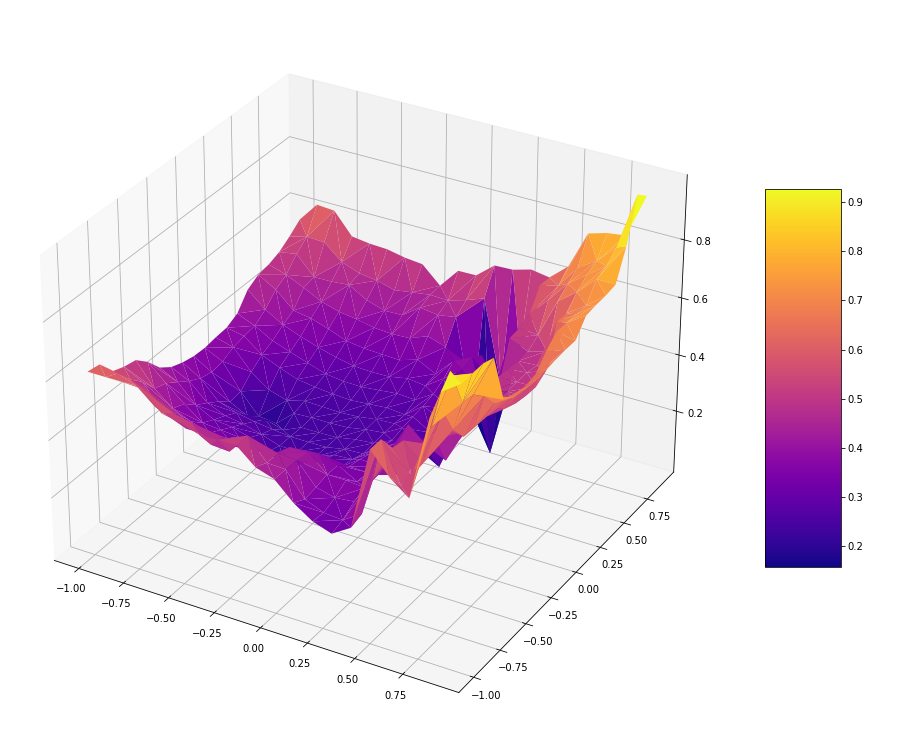
\includegraphics[scale=0.25]{figure/approximate}
			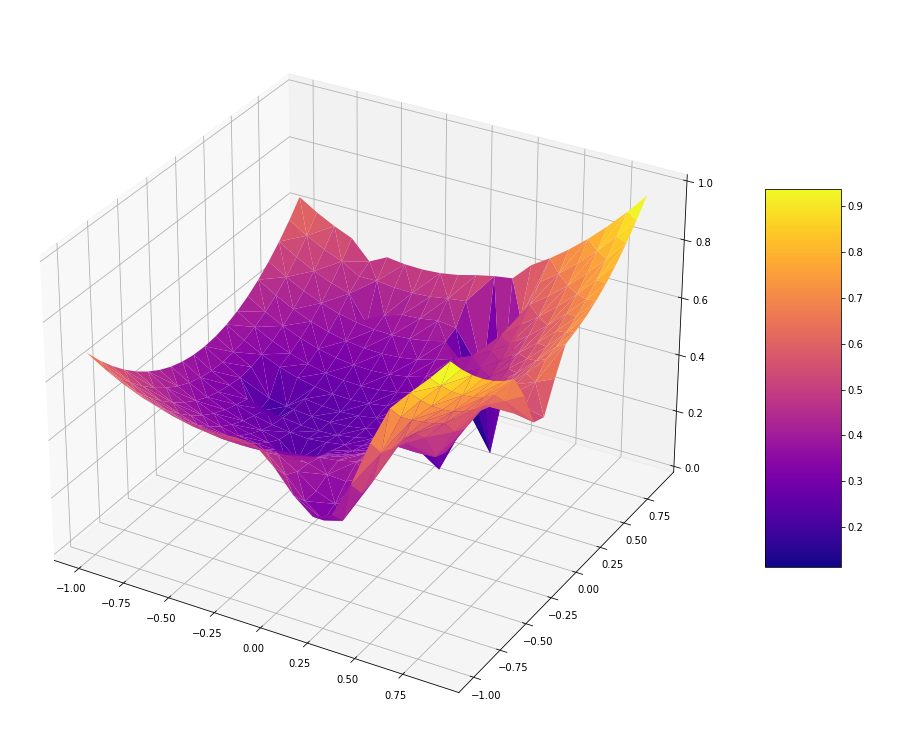
\includegraphics[scale=0.25]{figure/true}			
			\caption{Пример аппроксимированной (слева) и истинной (справа) функции из класса GKLS} %% подпись к рисунку
            \label{fio_ris1}
	\end{center}
\end{figure}


Для аппроксимации была выбрана нейронная сеть прямого распространения сигнала с 5-ю слоями по 32 нейрона в каждом. В качестве активационной функции в каждом нейроне была выбрана логистическая функция. 

Для обучения нейронной сети использовался заранее подготовленный набор из 160 точек испытания распределенных в области поиска.
Значения функции приводились к диапазону [0,1] перед обучением, аппроксимация также строилась в диапазоне [0,1].


После аппроксимации модель (нейронная сеть) передавалась в метод глобальной оптимизации.
В качестве такого метода использовался метод имитации отжига\cite{fio_bib7}.


Программная реализация аппроксимации функции с помощью нейронной сети проведена в среде Jupyter Notebook (сервис для интерактивных вычислений). В качестве языка программирования использован Python, который удобен для математических вычислений. Были задействованы следующие библиотеки языка Python: Numpy, Matplotlib, SciPy, Keras.


Алгоритм решения задачи оптимизации заключался в последовательном вызове алгоритма оптимизации на аппроксимированной функции и аппроксимации функции нейронной сетью \cite{fio_bib8}. В качестве критерия остановки использовалась близость найденной точки к априори известному минимуму.

Как показали проведенные эксперименты, использование нейросетевой аппроксимации позволяет сократить число вычислений целевой функции в 80\% задач.



\begin{biblio}

\bibitem{fio_bib1} Cybenko, G. V. Approximation by Superpositions of a Sigmoidal function. Mathematics of Control Signals and Systems. — 1989. — Т/. 2, № 4. — С. 303—314.

\bibitem{fio_bib2} Warren S. McCulloch, Walter Pitts // California State University. – Режим доступа:https://home.csulb.edu/~cwallis/382/readings/482/mccolloch.logical.calculus.ideas.1943.pdf 

\bibitem{fio_bib3} Paul Werbos // National Science Foundation. – Режим доступа: \url{https://www.researchgate.net/publication/35657389_Beyond_regression_new_tools_for_prediction_and_analysis_in_the_behavioral_sciences}

\bibitem{fio_bib4} Y.LeCun, B.Boser // ATI\&T Bell Laboratories. – Режим доступа: \url{http://yann.lecun.com/exdb/publis/pdf/lecun-89e.pdf}

\bibitem{fio_bib5} Sergeyev Y.D., Kvasov D.E. Diagonal'nyye metody global'noy optimizatsii. Fizmatlit, 2008. P. 352.

\bibitem{fio_bib6} Gaviano M., Lera D., Kvasov D. E., Sergeyev Y. D. Software for generation of classes of test functions with known local and global minima for global optimization // ACM Transactions on Mathematical Software. 2003. Vol. 29. P. 469-480.

\bibitem{fio_bib7} Kirkpatrick, S.; Gelatt Jr,C.D.;Vecchi, M. P. (1983). "Optimization by Simulated Annealing". Science. 220 (4598): 671–680.

\bibitem{fio_bib8} Мордухович Б. Ш. Методы аппроксимаций в задачах оптимизации и управления / Мордухович Б. Ш. . – М.: «Наука», 1988. – 360 c.

\end{biblio}

\msc{Код MSC2010}





\end{document}

